%% Be sure to check spelling!

%% Put your name and the proper due date in place

%% Note that the \includegraphics and \lstinputlisting commands
%% are currently commented out with %%% - until the
%% files exist, processing this code without them will result in an error
%% so leave the comments until you have created the files!

\documentclass{article}
\usepackage{amsmath}    % loads AMS-Math package
\usepackage{graphicx}   % bring in graphics
\usepackage{listings}   % allows lstlisting environment
\usepackage{moreverb}   % allows listinginput environment
\usepackage[letterpaper, margin=0.5in]{geometry}  % set paper size/margins
\usepackage{EGR103style}  % colorful file imports

\begin{document}
\begin{center}
\rule{6.5in}{0.5mm}\\~\\
\textbf{\large EGR 103L -- Fall 2021}\\~\\
\textbf{\huge Laboratory 10 - Optimization}\\~\\
**NAME (NET ID)**\\
Lab Section **NUMBER AND LETTER**, **DAY AND TIMES**\\
**DATEDUE**, **YEAR**\\~\\
{\small I have adhered to the Duke Community Standard in completing this assignment.  I understand that a violation of the Standard can result in failure of this assignment, failure of this course, and/or suspension from Duke University.} 
\rule{6.5in}{0.5mm}\\
\end{center}
\tableofcontents
\listoffigures
\renewcommand{\arraystretch}{1.5}
\clearpage

\section{Chapra 15.11}
The model equation is:
\begin{align*}
P&=P_m\frac{I}{I_{sat}}e^{-\frac{I}{I_{sat}}+1}=
~~~\frac{I}{~~~}e^{-\frac{I}{~~~}+1}
\end{align*}
with $P_m$ measured in (mg m$^{-3}$ d$^{-1}$) and $I_{sat}$ measured
in ($\mu$E m$^{-2}$ s$^{-1}$).
The statistical and information required by the problem is:
\begin{center}
\begin{tabular}{c|c|c}
$S_t$ & $S_r$ & $r^2$\\ \hline
~~~ & ~~~ & ~~~ \\
\end{tabular}
\end{center}
%%% Replace ~~~ above
%%% Discussion

\section{Chapra 15.22}
The model equation is:
\begin{align*}
y=\left(\frac{a+\sqrt{x}}{b\sqrt{x}}\right)^2
\end{align*}
where $a=~~~$ and $b=~~~$. The statistical and information required by the problem is:
\begin{center}
\begin{tabular}{c|c|c}
$S_t$ & $S_r$ & $r^2$\\ \hline
~~~ & ~~~ & ~~~ \\
\end{tabular}
\end{center}
This model predicts $y(1.6)=~~~$.
%%% Replace ~~~ above

\section{Chapra 15.29}
The model equation is:
\begin{align*}
\ln(p)=A-\frac{B}{C+T}
\end{align*}
where $A=~~~$, $B=~~~$, and $C=~~~$.  The statistical and information required by the problem is:
\begin{center}
\begin{tabular}{c|c|c|c}
$S_t$ & $S_r$ & $r^2$ & $s_{y/x}$\\ \hline
~~~ & ~~~ & ~~~ & ~~~ \\
\end{tabular}
\end{center}
%%% Replace ~~~ above

\section{Chapra 7.16}
Using {\tt fminbound} yielded a thickness of ~~~ mm for a temperature of ~~~K while using {\tt fmin} yielded a thickness of ~~~ mm for the same temperature of ~~~ K.
%%% Replace ~~~ above

\section{Chapra Problems 7.25, 7.26, and 7.27}
The required extremes are as follows:
\begin{itemize}
\item The minimum for 7.25 is $f(~~~, ~~~)=~~~$
\item The maximum for 7.26 is $f(~~~, ~~~)=~~~$.
\item The minimum for 7.27 is $f(~~~, ~~~)=~~~$.
\end{itemize}
%%% Replace ~~~ above

\section{Chapra 7.31}
Using {\tt fminbound} yielded a time of ~~~ days for an oxygen concentration of ~~~, while using {\tt fmin} yielded a time of ~~~ days for an oxygen concentration of ~~~.
%%% Replace ~~~ above

\section{Chapra 7.34}
Using {\tt fminbound} yielded a slip of ~~~ for a torque of ~~~, while using {\tt fmin} yielded a slip of ~~~ for a torque of ~~~. 
%%% Replace ~~~ above

\section{Chapra 7.36}
Using {\tt fminbound} yielded an $x$ of ~~~ for a function value of ~~~, while using {\tt fmin} yielded an $x$ of ~~~ for a function value of ~~~. 
%%% Replace ~~~ above

\pagebreak
\appendix
\section{Codes}
% Put the name of your file in the subsection name 
% and the listinginput input
% Be sure to include the community standard in codes!
% Add \clearpage commands if they make sense
% Make as many copies as you need
\lstset{style=python103, language=python} 

\subsection{Chapra 15.11}
%%%\lstinputlisting{chapra_15_011.py}
\clearpage

\subsection{Chapra 15.22}
%%%\lstinputlisting{chapra_15_022.py}
\clearpage

\subsection{Chapra 15.29}
%%%\lstinputlisting{chapra_15_029.py}
\clearpage

\subsection{Chapra 7.16}
%%%\lstinputlisting{chapra_7_016.py}
\clearpage

\subsection{Chapra 7.25-27}
%%%\lstinputlisting{extremes.py}
\clearpage

\subsection{Chapra 7.31}
%%%\lstinputlisting{chapra_7_031.py}
\clearpage

\subsection{Chapra 7.34}
%%%\lstinputlisting{chapra_7_034.py}

\subsection{Chapra 7.36}
%%%\lstinputlisting{chapra_7_036.py}
\pagebreak

\section{Figures}
% Make as many as needed; change sizes if it makes sense to do so
\begin{figure}[h!]
\begin{center}
%%%\includegraphics{chapra_15_011_plot.png}
\caption{Chapra 15.11}
\end{center}
\end{figure}

\begin{figure}[h!]
\begin{center}
%%%\includegraphics{chapra_15_022_plot.png}
\caption{Chapra 15.22}
\end{center}
\end{figure}

\begin{figure}[h!]
\begin{center}
%%%\includegraphics{chapra_15_029_plot.png}
\caption{Chapra 15.29}
\end{center}
\end{figure}
 
\begin{figure}[h!]
\begin{center}
%%%\includegraphics{chapra_7_016_plot.png}
\caption{Chapra 7.16}
\end{center}
\end{figure}
 
\begin{figure}[h!]
\begin{center}
%%%\includegraphics{chapra_7_025_plot.png}
\caption{Chapra 7.25}
\end{center}
\end{figure}
 
\begin{figure}[h!]
\begin{center}
%%%\includegraphics{chapra_7_026_plot.png}
\caption{Chapra 7.26}
\end{center}
\end{figure}
 
\begin{figure}[h!]
\begin{center}
%%%\includegraphics{chapra_7_027_plot.png}
\caption{Chapra 7.27}
\end{center}
\end{figure}
 
\begin{figure}[h!]
\begin{center}
%%%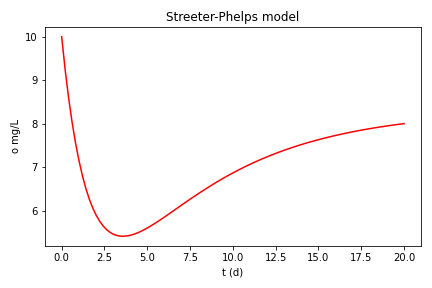
\includegraphics{chapra_7_031_plot.png}
\caption{Chapra 7.31}
\end{center}
\end{figure}

\end{document}
